%!TEX root = Slic3r-Manual.tex

\section{Hauteur de couche variable} % (fold)
\label{sec:variable_layer_height}
\index{layer height}
\index{hauteur de couche}

Slic3r donne la possibilit\'e de r\'egler la hauteur de couche entre des positions arbitraires le long de l'axe Z. Voil\`a, des parties du mod\`ele peuvent \^etre imprim\'es avec une hauteur de couche grossi\`ere, par exemple des sections verticales, et d'autres parties pourraient \^etre imprim\'es avec une hauteur de couche plus fine, par exemple les d\'egrad\'es inclin\'es o\`u les couches apparaissent plus marqu\'ees.

Le mod\`ele de la fig. \ref{fig:example_model} donne un exemple rudimentaire o\`u des hauteurs de couche variables pourraient \^etre utilis\'ees pour am\'eliorer la qualit\'e d'impression.  Les murs de la structure n'ont pas \`a \^etre imprim\'es en haute d\'efinition pour une qualit\'e acceptable, mais la pente du toit apparait en escalier, une hauteur de couche de 0,4 mm est trop grossi\`ere, en particulier pour la couche sup\'erieure, qui est aplatie.  Ceci est illustr\'e dans le G-Code repr\'esent\'e \`a la fig \ref{fig:example_gcode_normal_layer_heights}.


\begin{figure}[H]
\centering
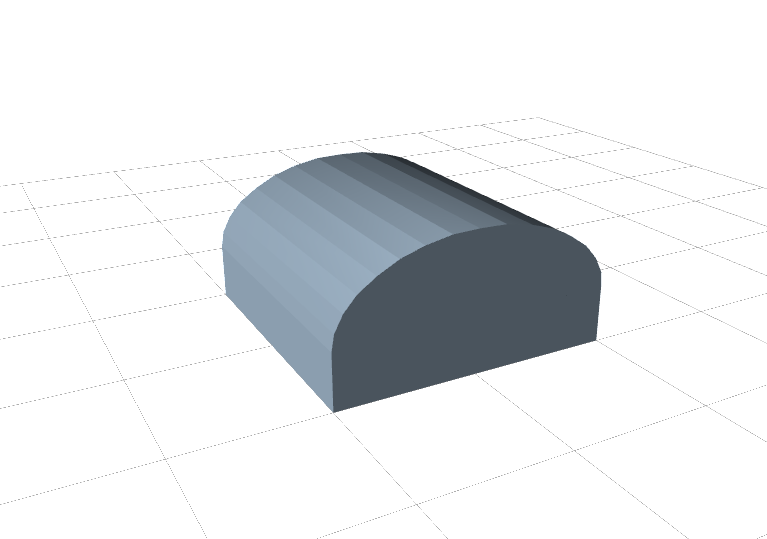
\includegraphics[keepaspectratio=true,width=0.75\textwidth]{expertmode/variable_layer_height/example_model.png}
\caption{Exemple de mod\`ele mettant en evidence un cas d'utilisation des couches variables.}
\label{fig:example_model}
\end{figure}

\begin{figure}[H]
\centering
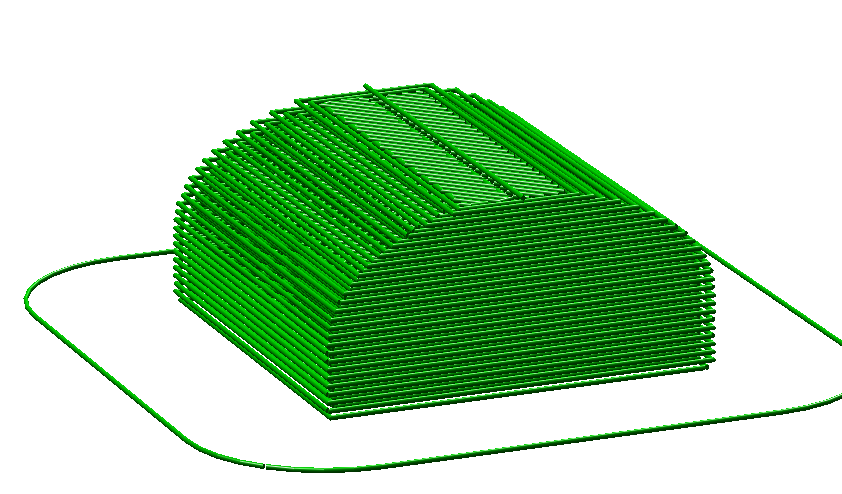
\includegraphics[keepaspectratio=true,width=0.75\textwidth]{expertmode/variable_layer_height/example_gcode_normal_layer_heights.png}
\caption{Exemple avec des couches normales.}
\label{fig:example_gcode_normal_layer_heights}
\end{figure}

Les param\`etres de hauteur de couche variables sont disponibles en double-cliquant sur ​​le nom de la pi\`ece dans la fen\^etre Plater (surface de travail).  Cela ouvrira une fen\^etre qui contient deux onglets. Le premier donne des informations sur le mod\`ele, comme indiqu\'e dans la fig. \ref{fig:variable_layer_height_options_tab_1}.

\begin{figure}[H]
\centering
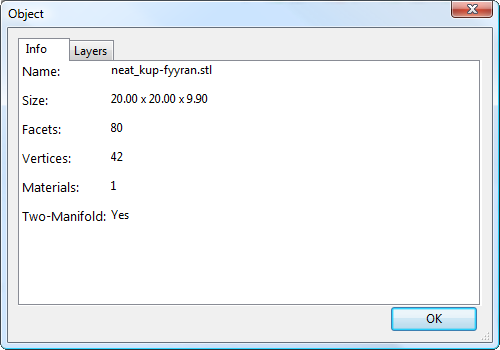
\includegraphics[keepaspectratio=true,width=0.75\textwidth]{expertmode/variable_layer_height/variable_layer_height_options_tab_1.png}
\caption{Param\`etres de Couche variable - Info.}
\label{fig:variable_layer_height_options_tab_1}
\end{figure}

Il convient de noter la hauteur du mod\`ele, puisque cela sera utile pour le calcul de la hauteur maximale de Z.

Le deuxi\`eme onglet (fig. \ref{fig:variable_layer_height_options_tab_2}) pr\'esente un tableau dans lequel chaque rang\'ee d\'efinit une hauteur de couche pour une plage particuli\`ere le long de l'axe Z, exprim\'ee en millim\`etres. Dans cet exemple, les parois du mod\`ele sont imprim\'ees \`a 0,4 mm, les parties raides du toit sont imprim\'ees \`a 0,2 mm, et la moins raide \`a 0,15 mm. Notez que chaque plage se divise exactement par la hauteur de la couche donn\'ee de sorte qu'il n'y a pas de «trous» entre les sections.

\begin{figure}[H]
\centering
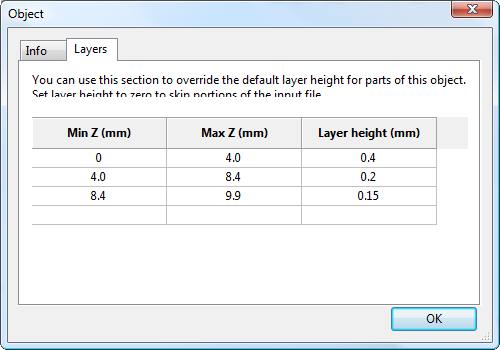
\includegraphics[keepaspectratio=true,width=0.75\textwidth]{expertmode/variable_layer_height/variable_layer_height_options_tab_2.png}
\caption{Param\`etres de Couche variable - Layers (Couches).}
\label{fig:variable_layer_height_options_tab_2}
\end{figure}

Le G-Code r\'esultant (fig. \ref{fig:example_gcode_variable_layer_heights}) montre une plus haute d\'efinition qui devrait aboutir \`a une impression de qualit\'e sup\'erieure.

\begin{figure}[H]
\centering
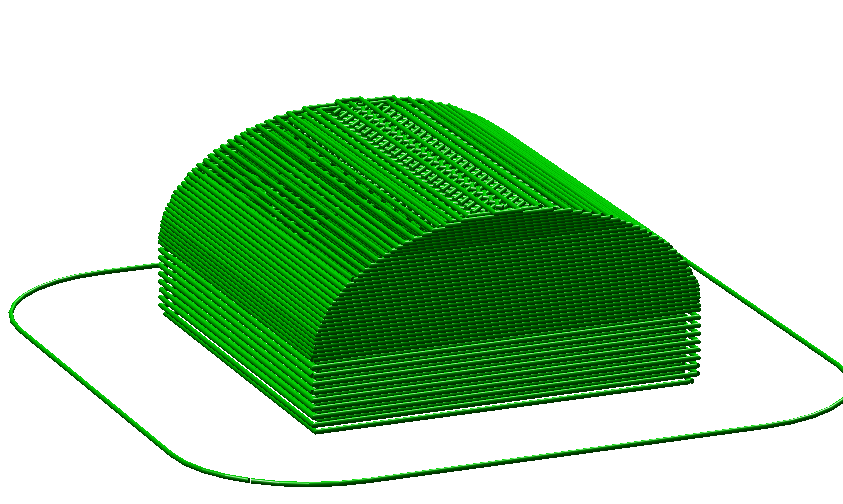
\includegraphics[keepaspectratio=true,width=0.75\textwidth]{expertmode/variable_layer_height/example_gcode_variable_layer_heights.png}
\caption{Example avec une hauteur de couche variable.}
\label{fig:example_gcode_variable_layer_heights}
\end{figure}

La Fig. \ref{fig:example_print} montre le mod\`ele d'exemple imprim\'e.  L'impression de gauche a 0,4 mm  de hauteur de couche partout, alors que l'impression de droite a une hauteur de couche variable.

\begin{figure}[H]
\centering
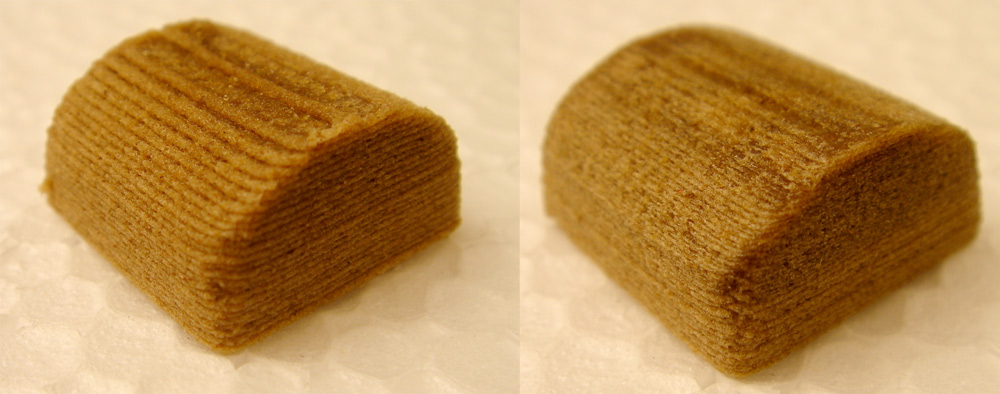
\includegraphics[keepaspectratio=true,width=1\textwidth]{expertmode/variable_layer_height/example_print.jpg}
\caption{Exemple d'impression avec une hauteur de couches variable.}
\label{fig:example_print}
\end{figure}

Une caract\'eristique suppl\'ementaire de l'option de hauteur de couches variable est que par la saisie d'un z\'ero pour une plage de la partie du mod\`ele ne sera pas imprim\'e.  Fig. \ref{fig:example_gcode_skipped_layers} montre le G-Code o\`u des couches entre 0 et 4 mm sont ignor\'es. Il s'agit d'un moyen utile de diviser un grand mod\`ele en plusieurs sections plus courtes, qui peuvent \^etre imprim\'es individuellement et assembl\'es par la suite.
\begin{figure}[H]
\centering
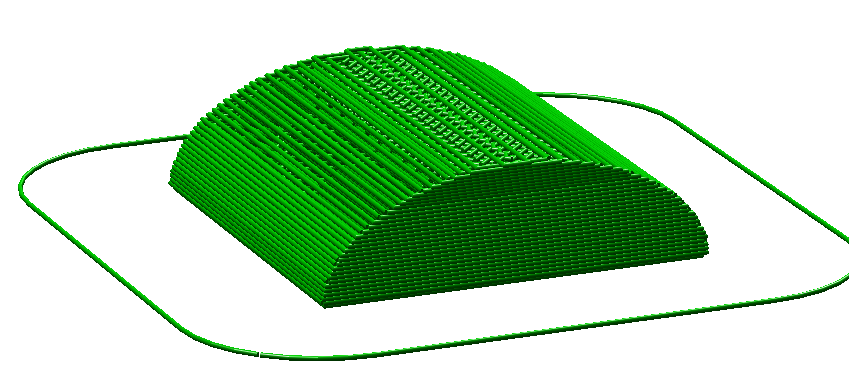
\includegraphics[keepaspectratio=true,width=0.75\textwidth]{expertmode/variable_layer_height/example_gcode_skipped_layers.png}
\caption{Exemple avec des couches ignor\'ees.}
\label{fig:example_gcode_skipped_layers}
\end{figure}

% section variable_layer_height (end)